\chapter{Advanced processes}
\label{sec:advanced}
\index{example processes!advanced}

At this point, we assume that you are familiar with the simple example 
from section \ref{sec:firstexample}. 
You should know how to read a dataset from a file, what a learner and 
a model applier do, and how a cross-validation chain works.
These operators will be used frequently and without further explanation
in this chapter. After reading this chapter you should be able to understand
most of the sample process definitions provided in the \filename{sample} directory of
\rapidminer. You should have a look at these examples and play around to get
familiar with \rapidminer.



\section{Feature selection}
\label{sec:advanced_feature_selection}
\index{feature selection}
Let us assume that we have a dataset with numerous attributes. 
We would like to test, whether all of these attributes are really
relevant, or whether we can get a better model by omitting some of 
the original attributes.
This task is called {\em feature selection} and the 
{\em backward elimination} algorithm is an approach that can 
solve it for you. 

Here is how backward elimination works within \rapidminer:
Enclose the cross-validation chain by a \op{FeatureSelection} 
operator. This operator repeatedly applies the cross-validation chain,
which now is its inner operator, until the specified stopping
criterion is complied with. The backward elimination approach
iteratively removes the attribute whose removal yields the largest
performance improvement. The stopping criterion may be for example 
that there has been no improvement for a certain number of steps. See
section \ref{sec:op:FeatureSelection} for a detailed description of
the algorithm. Figure \ref{fig:advanced1} shows the configuration
file.

You should try some of the following things:

\begin{itemize}
  \item Use {\em forward selection} instead of backward elimination by
    changing the parameter value of \para{selection\_direction} from
    \parval{backward} to \parval{forward}.
    This approach starts with an empty attribute set and iteratively
    adds the attribute whose inclusion improves the performance the
    most.
  \item Use the \op{GeneticAlgorithm} operator for feature selection
    instead of the \op{FeatureSelection} operator (see section
    \ref{sec:op:GeneticAlgorithm}).
  \item Replace the cross validation by a filter based evaluation. The sample
  process \filename{FeatureSelectionFilter.xml} uses such a fast feature
  set evaluation.
  \item Compare the results of the three approaches above to the 
    \op{BruteForce} operator.
    The brute force approach tests all subsets of the original attributes,
    i.e. all combinations of attributes, to select an optimal subset.
    While this operator is prohibitively expensive for large attribute
    sets, it can be used to find an optimal solution on small attribute 
    sets in order to estimate the quality of the results of other
    approaches.
\end{itemize}

\examplefile{advanced1.xml}{advanced1}{A feature selection process}




\section{Splitting up Processes}
\index{model file}
\index{attribute set description file}
If you are not a computer scientist but a data mining user, you are
probably interested in a real-world application of \rapidminer. 
   May be, you have a small labeled dataset and would like to train
a model with an optimal attribute set. 
   Later you would like to apply this model to your huge unlabeled 
database.
   Actually you have two separate processes.

\subsection{Learning a model}
This phase is basically the same as described in the preceeding section.
   We append two operators to the configuration file that write the results
of the process into files.
   First, we write the attribute set to the file 
\filename{selected\_at\-tri\-butes.att} using an \op{AttributeSetWriter}.
   Second, we once again train a model, this time using the entire example
set, and we write it to the file \filename{model.mod} with help of a
   \op{ModelWriter}.
   For the configuration file see figure \ref{fig:advanced2}. 
Execute the process and take a look at the file \filename{attributes.att}.
It should contain the selected subset of the originally used attributes, 
one per line.

\examplefile{advanced2.xml}{advanced2}{Training a model and writing it
to a file}

\subsection{Applying the model}
In order to apply this learned model to new unlabeled dataset, you
first have to load this example set as usual using an \op{ExampleSource}.
   You can now load the trained model using a \op{ModelLoader}.
Unfortunately, your unlabeled data probably still uses the original 
attributes, which are incompatible with the model learned on the
reduced attribute set.
   Hence, we have to transform the examples to a representation
that only uses the selected attributes, which we saved to the file 
\filename{attributes.att}.
   The \op{AttributeSetLoader} loads this file and generates (or rather
selects) the attributes accordingly.
   Now we can apply the model and finally write the labeled data 
to a file.
See figure \ref{fig:advanced3} for the corresponding configuration file. 

As you can see, you can easily use different dataset source files even in
different formats as long as you use consistent names for the attributes. 
You could also split the process into three parts:
\begin{enumerate}
  \item Find an optimal attribute set and train the model.
  \item Generate or select these attributes for the unlabeled data and
    write them to temporary files.
  \item Apply the model from step one to the temporary files from step
    two and write the labeled data to a result file.
\end{enumerate}

Of course it is also possible to merge all process modules into one big
process definition.

\examplefile{advanced3.xml}{advanced3}{Applying the model to unlabeled
data}




\section{Parameter and performance analysis}
\index{analysis}
\label{sec:parameter_optimization}
In this section we show how one can easily record performance values
of an operator or operator chain depending on parameter values. 
In order to achieve this, the \rapidminer process setup described in
this section makes use of two new \rapidminer operators: 
\refop{GridParameterOptimization} and \refop{ProcessLog}.

We will see how to analyze the performance of a support vector machine
(SVM) with a polynomial kernel depending on the two parameters 
degree $d$ and $\varepsilon$.\footnote{The performance of a polynomial
SVM also depends on other parameters like e.g. $C$, but this is not
the focus of this process.}

We start with the building block we should now be familiar with: a validation
chain containing a \op{LibSVMLearner}, a \op{ModelApplier}, and a
\op{PerformanceEvaluator}. Now we would like to vary the parameters.

Since we want to optimize more than one parameter, we cannot pass this
information to the \op{GridParameterOptimization} operator using the usual
\tag{<parameter>} tag. As the latter is designed to take a single
value, we must use the \tag{<list>} tag, which can take several
parameters. Similar to the \tag{<parameter>} tag the \tag{<list>} tag
must have a key. In case of the \op{GridParameterOptimization} this key is
(slightly confusingly in this context) named \para{parameters} (the
list of parameters which should be optimized). Each parameter 
that might be optimized, needs a \tag{<parameter>} tag entry in the \tag{<list>}.
The \tag{key} of a  \tag{<parameter>} tag has the form
\parval{OperatorName.parameter\_name} and the \tag{value} is a comma
separated list of values. In our case, the operator is named
"Training" and the parameters are \para{degree} and
\para{epsilon}. This leads to the following xml fragment:
\medskip

\begin{lstlisting}[style=rapidminerxmlstyle]{}
<list key="parameters">
  <parameter key="Training.degree" value="1,2,3,4"/>
  <parameter key="Training.epsilon" value="0.01,0.03,0.05,0.1"/>
</list>
\end{lstlisting}

Figure \ref{fig:advanced4} shows the entire example process setup.

\examplefile{advanced4.xml}{advanced4}{Parameter and performance analysis}

In GUI mode you do not have to bother about the XML code, just click
on the \useroption{Edit List} button next to the \para{parameters}
parameter of the \op{GridParameterOptimization} operator and add the two
parameters to the list.

If the value lists hold $n_1$ and $n_2$ values, respectively, the
\op{GridParameterOptimization} will apply its inner operators $n_1\cdot
n_2$ times. Finally the \op{GridParameterOptimization} operator returns an
optimal parameter value combination and the best performance
vector. If this is desired, the optimal parameter set can be written
to a file (for a specification see section
\ref{sec:parameter_set_files}) and reread from another process
using a \refop{ParameterSetLoader} and set using a
\refop{ParameterSetter}.
\medskip

In order to create a chart showing the absolute error over the parameters
$d$ and $\varepsilon$, we use the \op{ProcessLog} operator. Each time
this operator is applied, it creates a record containing a set of data
that we can specify. If the operator is applied $n$ times and we
specify $m$ parameters, we have a table with $n$ rows and $m$ columns
at the end of the process. Various plots and charts may be
generated from this table.

Similar to the optimization operator, the \op{ProcessLog} operator
accepts a \tag{<list>} of parameters specifying the values that should
be recorded. This list has the key \para{log}.
In our case, we are interested in three values: the values
of the parameters \para{degree} and \para{epsilon} and in the
performance of the models generated with these parameters. Therefore,
we add one \tag{<parameter>} tag to the \para{log} parameter
\tag{<list>} for each value we are interested in. (Again, in GUI mode,
simply click on the \useroption{Edit List} button next to the
\para{log} parameter of the \op{ProcessLog} operator.) The keys of
the parameters nested in this list may have arbitrary values. They are
used as column names and labels in charts only. We choose ``degree'',
``epsilon'', and ``performance''. The value of the parameters
specifies, how to retrieve the values. They are of the form
\begin{center}
operator.OperatorName.\{parameter$|$value\}.Name\footnote{If you
  wonder why this string starts with the constant prefix ``operator'',
  this is because it is planned to extend the \op{ProcessLog}
  operator by the possibility to log values taken from an input object
  passed to the operator.}
\end{center}
Two types of values can be recorded:
\begin{enumerate}
\item parameters that are specified by the process configuration or
  varied by the \op{GridParameterOptimization} operator and
\item values that are generated or measured in the course of the process.
\end{enumerate}
\para{degree} and \para{epsilon} are parameters of the operator named
``Training''. The performance is a value generated by the operator named
``XValidation''. Hence, our parameter list looks like this:
\medskip

\begin{lstlisting}[style=rapidminerxmlstyle]{}
<list key="log">
  <parameter key="degree" 
     value="operator.Training.parameter.degree"/>
  <parameter key="epsilon" 
     value="operator.Training.parameter.epsilon"/>
  <parameter key="performance" 
     value="operator.XValidation.value.performance"/>
</list>
\end{lstlisting}
For a list of values that are provided by the individual operators,
please refer to the operator reference (chapter
\ref{sec:operatorreference}).

Some plots may be generated online by using the GUI. This includes color and
3D plots like the one shown in figure
\ref{fig:svm_degree_epsilon_chart}.


%\inputfile{svm_degree_epsilon.txt}{svm_degree_epsilon}{The performance of a SVM
%  ({\tt gnuplot} input data file automatically generated by \rapidminer )}{The
%  performance of a SVM}

\begin{figure}[htbp]
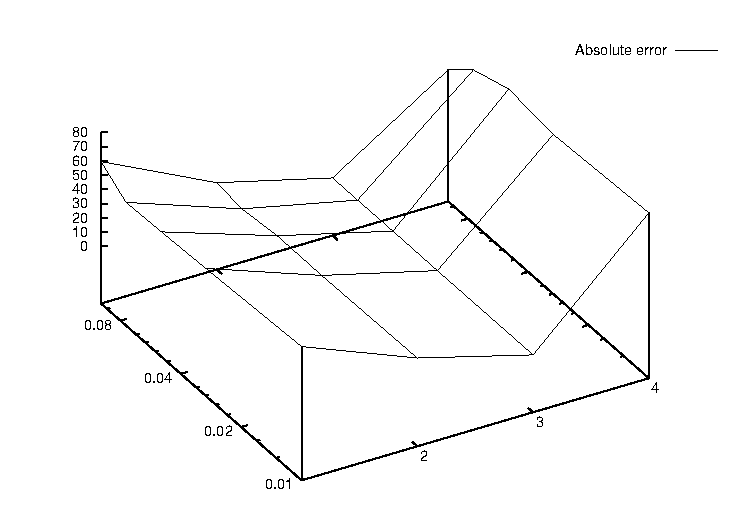
\includegraphics{graphics/svm_degree_epsilon.pdf}
\caption[Plot of the performance of a SVM]{The performance of a SVM (plot generated by {\tt gnuplot})}
\label{fig:svm_degree_epsilon_chart}
\end{figure}


\section{Support and tips}

\rapidminer is a complex data mining suite and provides a platform for a large
variety of process designs. We suggest that you work with some of the
building blocks described in this chapter and replace some operators and
parameter settings. You should have a look at the sample process definitions delivered
with \rapidminer and learn about other operators. However, the complexity of \rapidminer
might sometimes be very frustrating if you cannot manage to design the data
mining processes you want to. Please do not hesitate to use the user forum
and ask for help. You can also submit a support request. Both user forum
and support request tracker are available on our website
\begin{center}
\rapidminerurl
\end{center}
Beside this, we also offer services like support and consulting for our professional
users. Please contact us if you are interested in this form of professional support.

We conclude this chapter with some tips:
\begin{itemize}
\item You should make use of the automatic process validation available in
  the graphical user interface. This avoids a wrong process setup, missing
  parameter values, etc.
\item Work on a small subsample of your data during the process design and
  switch to the complete dataset if you are sure the process will properly
  run.
\item You do not have to write the attribute description files (XML) by
  hand. Just use the Attribute Editor of the GUI version or the configuration
  wizard of the \op{ExampleSource} operator.
\item Make use of breakpoints in the design phase. This helps to understand
  the data flow of \rapidminer and find potential problems, etc.
\item Start with small process setups and known building blocks and check if each
  new operator / operator chain performs in the way you have expected. 
\end{itemize}
